% Build: cd docs/talk && latexmk -pdf slides.tex   (figures: python3 ../figures/make_figures.py)
\documentclass[11pt,aspectratio=169]{beamer}
\usetheme[progressbar=frametitle, numbering=fraction, block=fill]{metropolis}
\usepackage[T1]{fontenc}
\usepackage{lmodern}
\usepackage{booktabs}
\usepackage{listings}
\usepackage{xcolor}
\usepackage{amsmath,amssymb}
\definecolor{kern}{HTML}{0072B2}
\definecolor{meas}{HTML}{E69F00}
\definecolor{pyiv}{HTML}{009E73}
\definecolor{trust}{HTML}{8C8C8C}
\setbeamercolor{alerted text}{fg=kern}
\setbeamercolor{progress bar}{fg=kern}
\setbeamercolor{frametitle}{bg=black!85}
\graphicspath{{../figures/}}
\lstset{basicstyle=\ttfamily\small, columns=fullflexible, keepspaces=true,
        keywordstyle=\color{kern}\bfseries, commentstyle=\color{black!55}, frame=none,
        literate={≤}{{$\le$}}1 {∈}{{$\in$}}1 {ℝ}{{$\mathbb{R}$}}1 {∧}{{$\wedge$}}1 {²}{{$^2$}}1}
\lstdefinelanguage{lean}{morekeywords={theorem,def,noncomputable,if,then,else,let,Icc},
  sensitive=true, morecomment=[l]{--}}
\lstdefinelanguage{f90}{morekeywords={if,then,else,endif},sensitive=false,morecomment=[l]{!}}
\newcommand{\ev}[1]{\textcolor{#1}{\rule{5pt}{5pt}}}
\newcommand{\take}[1]{\vfill\begin{center}\large #1\end{center}\vfill}

\title{Proving what a BerkeleyGW calculation computes}
\subtitle{A kernel-checked certificate for a G$_0$W$_0$--GPP run on Si-EPM, matched to 5\,$\mu$eV}
\author{Yizhou Wang \and Jinyuan Wu}
\institute{\footnotesize Formalization, certificates and analysis code written by Claude (Anthropic) under the authors' direction.\\
Reviewed by a separate AI reviewer (Codex); not a human-maintainer audit.}
\date{October 2026}

\begin{document}
\maketitle

% ------------------------------------------------------------------------------------------
\begin{frame}{The question}
\begin{columns}[c]
\begin{column}{0.6\textwidth}
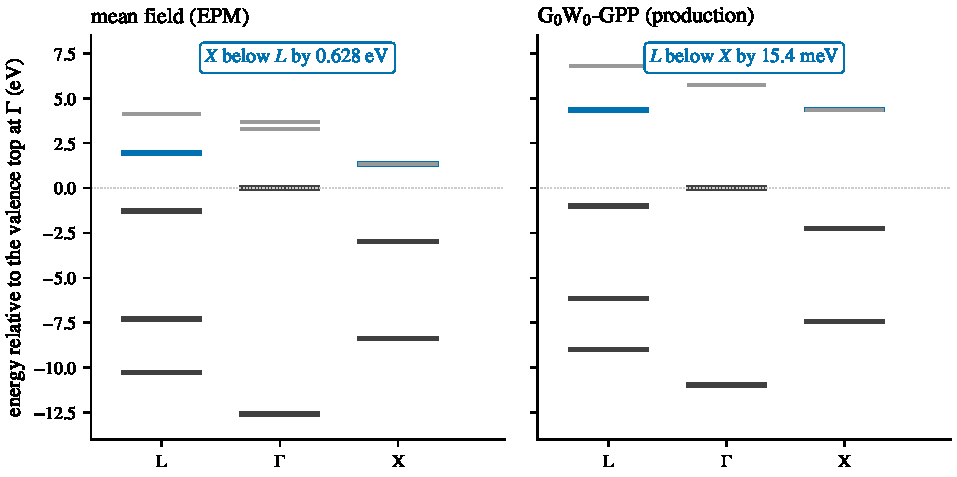
\includegraphics[width=\textwidth]{fig0_levels.pdf}
\end{column}
\begin{column}{0.38\textwidth}
BerkeleyGW's own \texttt{testsuite/Si-EPM}: G$_0$W$_0$ reverses the $X$/$L$ conduction ordering.

\vspace{4mm}
The flip is 15\,meV, out of self-energies of $\sim$9\,eV.

\vspace{4mm}
\alert{Is 15.4\,meV exactly what the code's equations give for this input?}
\end{column}
\end{columns}
\end{frame}

% ------------------------------------------------------------------------------------------
\begin{frame}{Three different questions}
\centering
\begin{tabular}{@{}lll@{}}
\toprule
 & question & here \\
\midrule
1 implementation & does the code compute its specified calculation? & \alert{\textbf{proved}} \\
2 convergence & is that calculation converged? & measured only \\
3 model & is G$_0$W$_0$/GPP the right physics? & not claimed \\
\bottomrule
\end{tabular}
\take{This talk is about layer 1, for one input deck.}
\end{frame}

% ------------------------------------------------------------------------------------------
\begin{frame}{Result}
\centering
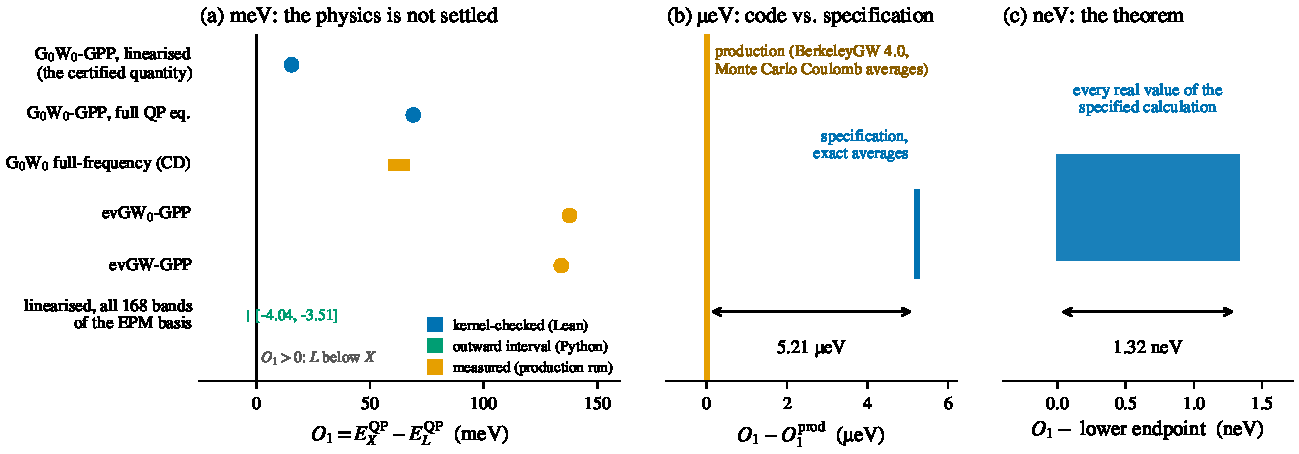
\includegraphics[width=\textwidth]{fig1_three_scales.pdf}
\vfill
\begin{tabular}{@{}rl@{}}
\ev{kern}\ Lean theorem, no hypotheses: & $O_1 \in [15.405752349,\ 15.405753673]$\,meV \\
\ev{meas}\ BerkeleyGW 4.0 prints: & $15.400547$\,meV \quad(5.21\,$\mu$eV away)
\end{tabular}
\end{frame}

% ------------------------------------------------------------------------------------------
\begin{frame}{What is proved, what is trusted}
\centering
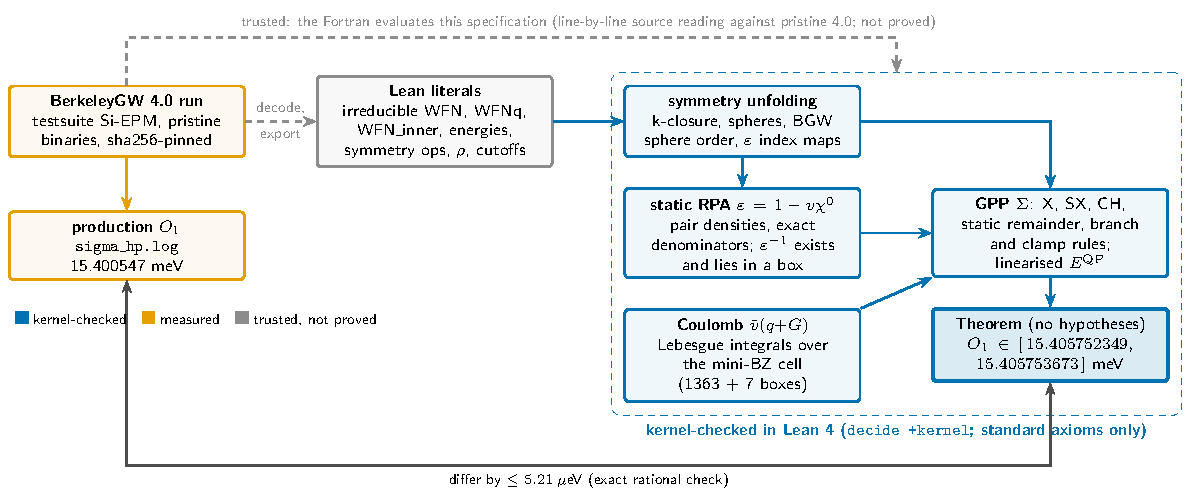
\includegraphics[width=\textwidth]{pipeline.pdf}
\end{frame}

% ------------------------------------------------------------------------------------------
\begin{frame}[fragile]{The theorem}
\begin{lstlisting}[language=lean]
theorem o1_enclosure_irr_unconditional :
    O1 glI stXI stLI EIrr vbTrue oqTrue ∈
      Icc ((8880811588953599 : ℝ) / 2 ^ 59) ((8880812351936001 : ℝ) / 2 ^ 59)
\end{lstlisting}
\vspace{3mm}
\begin{itemize}
\item \texttt{O1} is a real number: exact $\chi^0$, the true $\varepsilon^{-1}$, GPP $\Sigma$, linearised QP.
\item Inputs: the \emph{irreducible} wavefunctions; unfolding and Coulomb integrals are proved.
\item Kernel-checked (\texttt{decide +kernel}); only the three standard axioms.
\end{itemize}
\end{frame}

% ------------------------------------------------------------------------------------------
\begin{frame}[fragile]{The specification reads like \texttt{mtxel\_cor.f90}}
\textbf{BerkeleyGW 4.0}, occupied GPP branch
\begin{lstlisting}[language=f90,basicstyle=\ttfamily\normalsize]
if (wdiffr.gt.limittwo .and. delwr.lt.limitone) then
  sch = delw * I_eps_array(ig,my_igp)
\end{lstlisting}
\vspace{2mm}
\textbf{Lean}, \texttt{SigmaSpec.schM}
\begin{lstlisting}[language=lean,basicstyle=\ttfamily\normalsize]
if (x - w) ^ 2 > GAM2 ∧ w ^ 2 < (x - w) ^ 2 * LIM1
then w * IeU I / (x - w) else 0
\end{lstlisting}
\vfill
\small Division-free form, proved equal to the source's rule where that is defined. Every definition
sits next to its Fortran in \texttt{docs/review/index.html}. \textcolor{trust}{That correspondence is
read, not proved.}
\end{frame}

% ------------------------------------------------------------------------------------------
\begin{frame}{Where the 5.21\,$\mu$eV comes from}
\begin{itemize}
\item BerkeleyGW averages $8\pi/|q{+}G|^2$ over the mini-BZ by Monte Carlo; the proof uses the exact
      integrals. The averages differ by up to $1.7\times10^{-3}$.
\item Each $E^{\rm QP}$ moves by 0.14--0.18\,meV; in $O_1$ this cancels to 5.21\,$\mu$eV.
\item With BerkeleyGW's own Monte Carlo averages, an outward-rounded evaluator encloses every
      printed $E^{\rm QP}$.
\end{itemize}
\take{No implementation discrepancy on any active code path of this deck.}
\end{frame}

% ------------------------------------------------------------------------------------------
\begin{frame}{Documented conventions decide the sign}
\centering
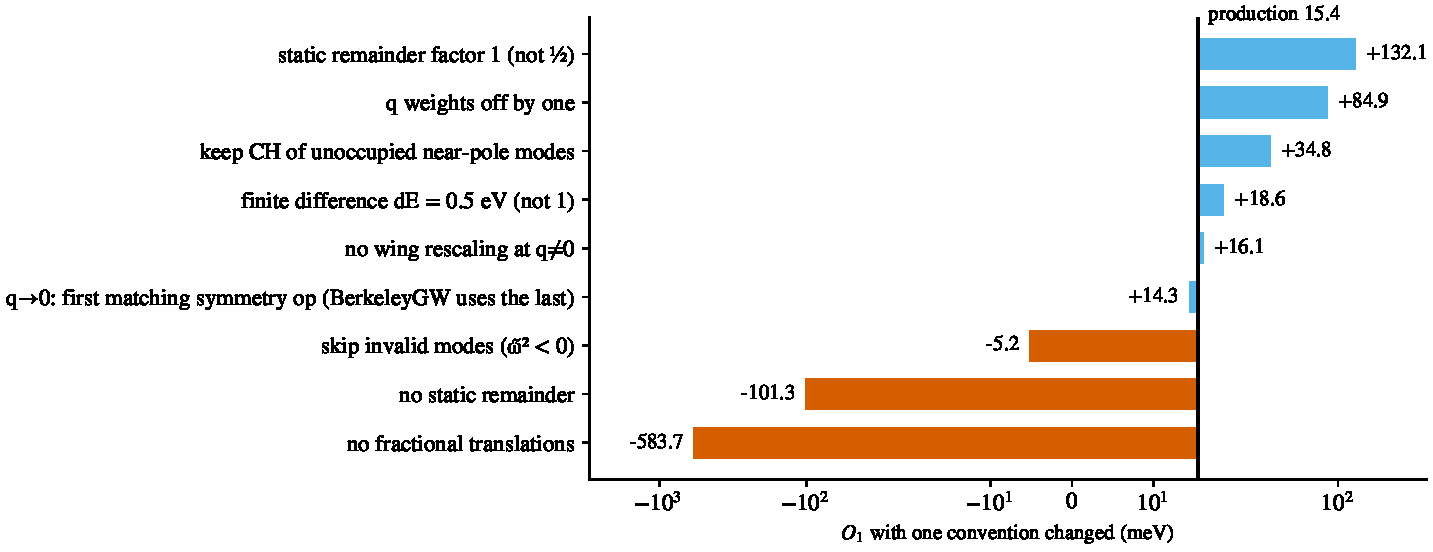
\includegraphics[width=0.9\textwidth]{fig2_conventions_slide.pdf}

\small Each bar changes one convention; all 15 changes are detected at $10^{-8}$\,eV in the $\Sigma$ table.
None is a bug.
\end{frame}

% ------------------------------------------------------------------------------------------
\begin{frame}{The $q\to0$ cell picks one direction}
\begin{itemize}
\item $\Sigma$ uses the \emph{last} matching symmetry operation for each $q$; at $q=0$ that fixes
      one direction of the anisotropic head and wings.
\item Over all directions: $O_1\in[14.34, 15.41]$\,meV. Direction average: 14.89\,meV.
\item Exactly degenerate states split; the $\Gamma$ valence SX$-$X spreads by 36\,meV before the
      multiplet average hides it.
\end{itemize}
\vfill
\scriptsize\textcolor{pyiv}{Outward-interval (Python) results, not kernel-checked.}
\end{frame}

% ------------------------------------------------------------------------------------------
\begin{frame}{Convergence: the sign comes from cancelling truncations}
\begin{columns}[c]
\begin{column}{0.6\textwidth}
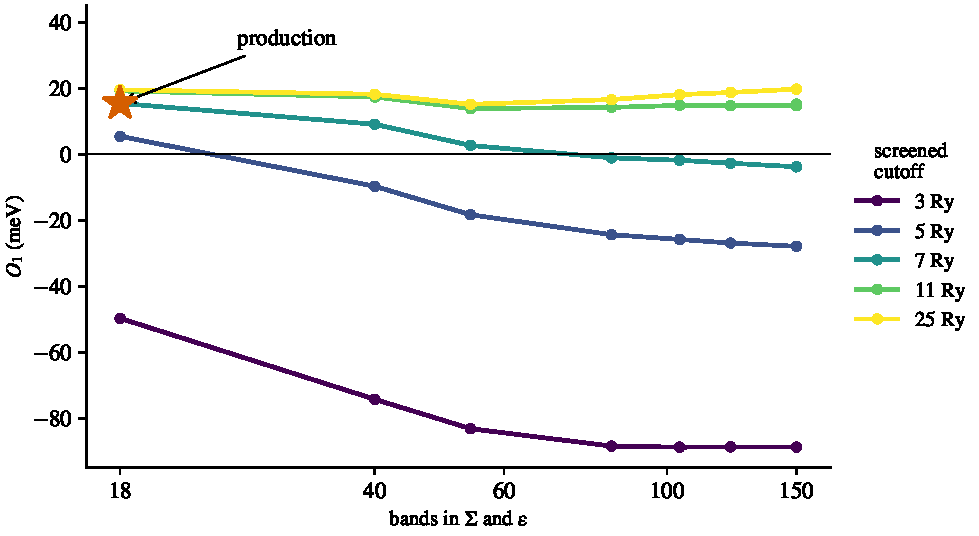
\includegraphics[width=\textwidth]{fig3_convergence_slide.pdf}
\end{column}
\begin{column}{0.38\textwidth}
At 7\,Ry, adding bands takes $O_1$ from $+15.4$ to $-3.8$\,meV.

\vspace{3mm}
At 18 bands, raising the cutoff looks converged.

\vspace{3mm}
\textcolor{meas}{125 production runs. Measured; no convergence claim.}
\end{column}
\end{columns}
\end{frame}

% ------------------------------------------------------------------------------------------
\begin{frame}{The GW hierarchy moves $O_1$ by tens of meV}
\begin{columns}[c]
\begin{column}{0.5\textwidth}
\begin{tabular}{@{}lr@{}}
\toprule
treatment & $O_1$ (meV) \\
\midrule
\ev{kern} G$_0$W$_0$-GPP, linearised & $+15.4$ \\
\ev{kern} G$_0$W$_0$-GPP, full QP & $+69.0$ \\
\ev{meas} full frequency (CD) & $+58$ to $+67$ \\
\ev{meas} evGW$_0$-GPP & $+137.9$ \\
\ev{meas} evGW-GPP & $+134.2$ \\
\bottomrule
\end{tabular}
\end{column}
\begin{column}{0.46\textwidth}
\small
\begin{itemize}
\item $V_{xc}=0$: QP energies sit $\sim$7\,eV from mean field, deep in $\Sigma$'s poles.
\item Proved: exactly two QP roots per state in $[-10^4,10^4]$\,eV; the principal one is unique only
      because of the \texttt{sexcut} clamp.
\item Plasmon-pole error at $E_o$: $-31.6$\,meV.
\end{itemize}
\end{column}
\end{columns}
\end{frame}

% ------------------------------------------------------------------------------------------
\begin{frame}{From theory to the specification}
\begin{itemize}
\item Proved under named hypotheses: the pole signs of $\Sigma$ from time-ordered $G_0$, the HL-GPP
      algebra and SX/CH split, the static RPA structure.
\item Every departure of code from theory is listed: \emph{proved equal} or \emph{named approximation}.
\item Formalization made three edge cases explicit:
  \begin{itemize}
  \item $x = 0$ exactly at $q = 0$ (\texttt{TOL\_Zero} substitution);
  \item the GPP kernel is discontinuous at $(x,\Omega^2)=(0,0)$;
  \item the one-system theorem cannot be applied at $X$ or $L$.
  \end{itemize}
\end{itemize}
\vfill
\scriptsize Conditional identities; not instantiated on the certified run.
\end{frame}

% ------------------------------------------------------------------------------------------
\begin{frame}{What is not claimed}
\begin{columns}[T]
\begin{column}{0.48\textwidth}
\begin{block}{Trusted, not proved}
\begin{itemize}
\item export of the run files into Lean
\item that the Fortran evaluates the specification
\item the production execution
\end{itemize}
\end{block}
\end{column}
\begin{column}{0.48\textwidth}
\begin{alertblock}{Not claimed}
\begin{itemize}
\item correctness on other inputs
\item convergence of 18 bands
\item that GW/GPP or the EPM describe Si
\item verification of BerkeleyGW's physics
\end{itemize}
\end{alertblock}
\end{column}
\end{columns}
\vfill
\small Trusted computing base: Lean 4.19 kernel, Mathlib, elan. No external re-checker run yet.
\end{frame}

% ------------------------------------------------------------------------------------------
\begin{frame}{What we would like from you}
\begin{enumerate}
\item \textbf{Does the specification match your reading of the code?}\\
      \small Every Lean definition is next to its Fortran lines in \texttt{docs/review/index.html}.
\item \textbf{What should come next?}\\
      \small LDA $V_{xc}$, complex flavour, full frequency, a 2D material with truncation.
\item \textbf{Would certified reference values help the testsuite?}\\
      \small The convention study already detects changes at $10^{-8}$\,eV.
\end{enumerate}
\end{frame}

% ------------------------------------------------------------------------------------------
\begin{frame}[fragile]{Reproduce}
\begin{columns}[c]
\begin{column}{0.5\textwidth}
\begin{lstlisting}
bash scripts/bootstrap.sh
bash scripts/verify.sh
\end{lstlisting}
\small Build, exhaustive axiom audit,\\ 699 scientific and 16 workflow tests;\\ about 5\,h from a cold build.
\end{column}
\begin{column}{0.46\textwidth}
\small
\begin{tabular}{@{}lr@{}}
\toprule
theorems audited & 34\,553 \\
certificate modules & 1\,376 \\
Coulomb boxes proved & 1\,363 + 7 \\
production runs & 125 \\
\bottomrule
\end{tabular}
\end{column}
\end{columns}
\vfill
\centering\small \texttt{github.com/MichealWangYZ/bgw-lean-certificate}
\end{frame}

% ------------------------------------------------------------------------------------------
\begin{frame}[standout]
The code computes what its source says,\\ to 5\,$\mu$eV, on this deck.\\[4mm]
\normalsize Convergence, the plasmon pole and the vertex remain physics.
\end{frame}

\appendix
\begin{frame}{References}
\small
\begin{itemize}
\item M.~S.~Hybertsen and S.~G.~Louie, Phys.\ Rev.\ B \textbf{34}, 5390 (1986).
\item J.~Deslippe \emph{et al.}, Comput.\ Phys.\ Commun.\ \textbf{183}, 1269 (2012).
\item B.-C.~Shih \emph{et al.}, Phys.\ Rev.\ Lett.\ \textbf{105}, 146401 (2010).
\item The Lean 4 theorem prover and Mathlib.
\end{itemize}
\end{frame}

\begin{frame}{Backup: evidence for each number}
\tiny
\begin{tabular}{@{}p{0.36\textwidth}p{0.22\textwidth}p{0.36\textwidth}@{}}
\toprule
number & evidence & where \\
\midrule
$O_1\in[15.405752349, 15.405753673]$ meV & \ev{kern} Lean & \texttt{Headline.o1\_enclosure\_irr\_unconditional} \\
$O_1 > 0$ & \ev{kern} Lean & \texttt{Headline.o1\_pos\_irr\_unconditional} \\
full-QP $O_1\in[68.9856742, 68.9856744]$ meV & \ev{kern} Lean & \texttt{Headline.o1\_fullQP\_irr\_unconditional} \\
5.21\,$\mu$eV & exact rationals & \texttt{tests/test\_endpoint\_e1.py} \\
$q\to0$ range, direction average & \ev{pyiv} interval & \texttt{bgw/endpoint/cert.py} \\
all-band $O_1\in[-4.05,-3.51]$ meV & \ev{pyiv} interval & \texttt{bgw/r28\_f3} \\
convention study & \ev{meas} reproducer & \texttt{data/mutations\_e1.log} \\
convergence, FF, evGW & \ev{meas} production & \texttt{docs/ENDPOINT.md} \\
\bottomrule
\end{tabular}
\end{frame}

\end{document}
